\documentclass{article}

\usepackage{fancyhdr}
\usepackage{graphicx}  % This package allows the importing of images
\graphicspath{ {./} }
\usepackage[margin=1in]{geometry}
\usepackage{mdframed}
\usepackage{enumitem}
\usepackage{amsfonts}
\usepackage{graphicx}
\usepackage{commath}
\usepackage{amssymb}
\usepackage{outlines}
\usepackage[dvipsnames]{xcolor}
\usepackage{multicol}
\pagestyle{fancy}
\usepackage{hyperref}

\newcommand{\maketitletwo}{
    
    \rhead{Aditya Tapshalkar \\ YOLOv4 GTSDB Evaluation}
    
    
    \begin{center}
        \Large{\textbf{Data Management and Analysis}}
        \vspace{5pt}
        \thispagestyle{empty}
        \normalsize{\\ Aditya Tapshalkar}
        \small{\\ Fall 2021 \\}            
    \end{center}
    \newpage
}

\begin{document}
    
    \maketitletwo
    
    \section{Abstract}
    
        This report details my procedures for database management and subsequent evaluation of this data. In this problem set, I will deal with the manipulation and evaluation of data and inclusion of additional classes from YOLOv3\cite{yolov3} detection data trained from various Chinese road sign databases, such as Tsinghua-Tencent 100K (TT100K)\cite{Zhe_2016_CVPR}, to the German Traffic Sign Detection Benchmark (GTSDB) dataset\cite{Houben-IJCNN-2013}. \\
        
        My results and code can be found at: \url{https://github.com/adityataps/YOLOv4-on-GTSDB}.
    
    \pagebreak
    
    \section{Methodology}
    
        The goal of this problem set is to showcase my skills in exploring how an existing dataset can be modified to accommodate for additional data and assessing the performance of a trained model from result data and modified ground truths. 
        
        \subsection{Task 1}
        
            This problem set consisted of two main tasks. The first task was to update the ground truths text file, provided by the GTSDB dataset, to account for two signs not originally annotated and recorded by the GTSDB team. These signs would be assigned to classes 43 and 44. 
            
            \begin{figure}[h!]
                \centering
                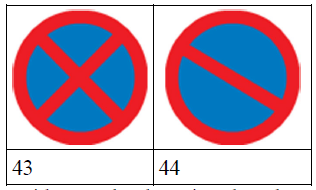
\includegraphics[scale=0.5]{pn_gtsdb}
                \caption{Classes 43 and 44, not previously included in the GTSDB dataset}
            \end{figure}
        
            A JSON file with predictions made by a YOLOv3 model trained with Chinese road sign datasets was provided to narrow down the number of images to annotate. While utilizing this JSON results file eliminated the need to view all 900 images in the GTSDB dataset, doing so naively assumes that the predictions are ground truths and images not predicted to contain these new signs strictly do not contain these signs. This can bring about the issue of not including false negatives (i.e. signs that were not detected). The only way all signs found in the GTSDB dataset are included in the ground truths text file is to manually analyze the entire dataset. 
            
            \begin{figure}[h!]
                \centering
                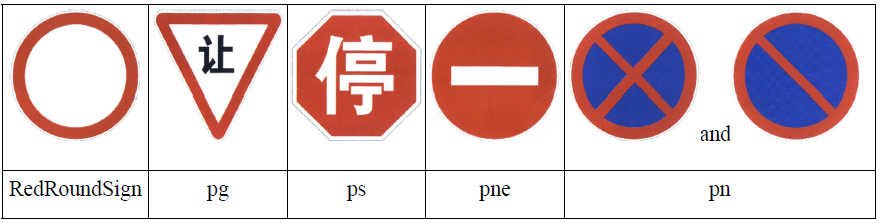
\includegraphics[scale=0.5]{json_classes}
                \caption{The YOLOv3 pre-trained model classes}
            \end{figure}
        
            The YOLOv3 model was trained with five classes in mind, as shown above. The "pn" class consists of both sign types, meaning that images with "pn" sign detection needed to be manually reviewed to determine whether the detected sign belonged to class 43 or 44. 
            
            A Python script was fabricated to naively append the GTSDB ground truths text file with classes 43 and 44. This script first parses the JSON file and gathers a list of images predicted to contain signs in the "pn" class and then asks the user to provide the class definition for each "pn" detection to provide annotations for the GTSDB ground truths file. The detection data is then formatted into GTSDB ground truth format. \\
            
            The JSON file can be found at: \url{https://www.dropbox.com/s/b9aootj3z9gl1vs/GTSDB.json?dl=0}. \\
            
        \subsection{Task 2}
        
            This task builds off the procedures conducted in Task 1 and deals with the evaluation of YOLOv3 model given the JSON predictions file and newly appended ground truth annotations file.
            
            To analyze detection data for all images, a mapping had to be created to build a relation between the classes in the GTSDB dataset and the classes used by the detector. 
            
            \begin{figure}[h!]
                \centering
                \begin{tabular}{c|c}
                    & \\
                    Detector classes & GTSDB classes \\
                    \hline
                    RedRoundSign & 0, 1, 2, 3, 4, 5, 6, 7, 8, 9, 10, 15, 16 \\
                    
                    pg & 13 \\
                    
                    ps & 14 \\
                    
                    pne & 17 \\
                    
                    pn & 43, 44 \\
                    
                \end{tabular}
                \caption{The mapping of GTSDB classes to detector classes}
            \end{figure}

            A second Python script was then written to evaluate the model on the GTSDB ground truths. Here, the true positives, false negatives, and false positives were counted for each image, after which the overall mean average precision, average precision and recall values, and F1 score were calculated. 
            
            \subsubsection{Results and Reflection}
                
                An issue I encountered and needed to address was how to deal with divisions by zero when there were zero true positives, false negatives, and false positives.
                
                I decided to record two evaluation files: one evaluation where values of 1 were appended to image-wise precision and recall values, as addressed and practiced by the General Entity Annotator Benchmark (GERBIL) \cite{DBLP:journals/semweb/RoderUN18}; and one evaluation where image-wise precisions and recalls with zero true positives, false negatives, and false positives were omitted due to inconclusive data. 
                
                In both evaluations, 618 true positives, 116 false negatives, and 34 false positives were observed. The average precision and recall for the entire dataset were roughly 0.948 and 0.842, and the F1 Score for the dataset was 0.892. The mean average precision for the first evaluation method mentioned above was 0.993, while the mean average precision for the latter evaluation was 0.954. The large number of overall false negatives and low total recall value indicate that the detector is consistently missing road signs that should be detected. 
                
                It is important to note that these results are based off incomplete ground truths generated from Task 1. Although the model recorded detections with a detection threshold of 0.50, discrepancies and low model reliability could create a large number of false negatives we could only count by manually processing the entire GTSDB dataset. Generating ground truths from prediction data and then evaluating the same data with the ground truths can cause biases in favor of the prediction data. Without accounting for false negatives for the "pn" class by the detector, we would mistakenly gather that the detector is exceptionally reliable at detecting "pn" signs. Therefore the confidence of "pn" sign detection cannot be determined until all "pn" false negatives are also appended to the ground truths. 
                
                To improve the detector to get better results, I would take a closer look at the dataset and ensure that no false negatives would be omitted from the ground truths. Without directly analyzing the GTSDB dataset one image at a time, I believe improving the training dataset for the YOLOv3 detector, perhaps by including more training images, would drastically increase my confidence in "pn" sign detection. 
                
                In all, the utilization of the detector JSON data helped efficiently add annotations to the ground truths but naively introduced uncertainty as to whether other images included "pn" signs that were not detected by the model. These annotations could be used for training, but creates bias favoring the model's detection data and may cause overfitting. Some ways I believe could improve the training process would be to manually analyze each image in the entire dataset, or utilize an even more exhaustive dataset for the model to further improve detection (but this can still cause bias). 
                
        
    
    \pagebreak
    \bibliography{references}
    \bibliographystyle{acm}
    
    
    
\end{document}